\chapter{Experiment Setup}
\section{RHIC}
The Relativistic Heavy Ion Collider (RHIC) is a superconducting charged hadron collider located at Brookhaven National Lab (BNL) in Upton, NY, United States. RHIC is capable of accelerating heavy ions such as Au (gold) or Cu (copper) nuclei to energies of $\sim$100 GeV per nucleon. RHIC is also capable of accelerating lighter ions such as protons, deuteron, and helium to $\sim	$100 GeV per nucleon and $\sim$250 GeV per proton, in the case of \pp. The machine has been demonstrated the ability to reliably create the so called QGP (Quark Gluon Plasma) matter.

There are two major detector experiments currently operating in interaction regions around the RHIC ring: PHENIX (Pioneering High Energy Nuclear Interaction eXperiment) and STAR (Solenoidal Tracker at RHIC). Figure \ref{fig:rhic_heli_photo} shows the locations of the experiments and the accelerator chain. A typical schedule for RHIC is to operate the accelerator for 32 cryo-weeks every year in what is called a ``Run." There have been 16 Runs so far but the relevant Run for this thesis was the 15th Run taken in 2015 which ran proton colliding with gold ions (\pau) \sqsn = 200 GeV for part of its running. Specific details about this dataset are found in Section \ref{sec:Run_15}.

\begin{figure}[!ht]
\centering
\includegraphics[width=0.65\linewidth]{figs/rhic-map.png}
\caption{A helicopter's view of the accelerator chain in BNL starting at the Tandems (in gold) and ending at the RHIC ring (in blue and yellow for the two counter-circulating beams). STAR and PHENIX can be seen at two of the interaction regions. The ring is 2.38 miles in circumference~\cite{Tannenbaum:2013wkn}.}
\label{fig:rhic_heli_photo}
\end{figure}

The RHIC ring is at the end of a chain of smaller accelerators that are used to ``feed" the ions into the RHIC ring, where they are accelerated (or decelerated in some circumstances) to the desired collision energy. For heavy ions such as Au, the process of production and acceleration is listed in detail below \cite{ROSER200223}.
%\textbf{TO DO modify to included EBIS instead of Tandem!}
\begin{enumerate}
  \item{} A pulsed sputter Au ion source generates negative ions in the Tandem Van De Graaff.
  \item{} The ions are passed through an electron stripping foil to achieve a positive +12 $e$ charge and accelerated to $\sim$1 MeV per nucleon.
  \item{} The ions pass through bending magnets and another foil to further strip electrons and filter charge, yielding to a positive +32 $e$ charge state.
  \item{} The ions are sent to the Booster Synchrotron, which accelerates them to 95 MeV per nucleon and leaves them at a positive +77 $e$ charge.
  \item{} The ions enter the Alternating Gradient Synchrotron (AGS) in bunches of 24 around the ring. The ions are debunched and rebunched into four bunches and then accelerated to 10.8 GeV per nucleon.
  \item{}  The bunches then exit the AGS one at a time, where their Au ions are stripped of their two remaining electrons, yielding a final charge state of positive +79 $e$. Finally, the bunches are transferred to their respective buckets in RHIC. 
\end{enumerate}

For protons, the process instead begins at the Linear Accelerator (LINAC) facility. The protons are then sent through the chain of accelerators in a similar way to the heavy ions until reaching RHIC in either a polarized or unpolarized spin state. 

Once the ions have reached RHIC, they will enter one of two independent rings, blue or yellow, each circulating in an opposite direction. The ions in the rings are deflected and focused by 1,740 superconducting magnets using niobium-titanium conductors. Once the ions are focused and accelerated to the desired parameters around the RHIC, the ions are deflected into the six interaction regions where the blue and yellow rings intersect to produce collisions. It is at these interaction regions where the major experiments have set up their detectors, with STAR at the 6 o'clock position and PHENIX at the 8 o'clock position.

The period of time that collisions continue is known as a ``fill," and the average length of a fill is eight hours. As the fill wears on, the collision rate substantially decreases as the density of ions in the machine decreases. Once the collision rate has been reduced sufficiently, it is more efficient to start the fill over at a higher collision rate.  

%Electron cooling was implemented in RHIC to increase the luminosity of fills and slow the luminosity decay. The basic concept of electron cooling is to shoot electrons at the heavy ion beams in RHIC 
%\begin{figure}[!h]
%\begin{center}
%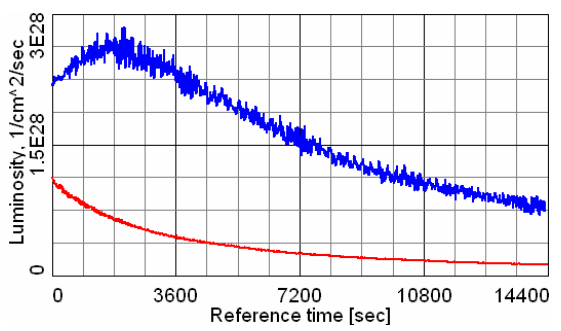
\includegraphics[width=0.5\linewidth]{figs/rhic_electron_cooling_sim.png}
%\caption{The luminosity vs time for Au-Au at 200 GeV simulations with (blue) and without (red) electron cooling. Electron cooling is shown to be an effective way of increasing luminosity in simulations. ~\cite{fedotov2007progress}}
%\end{center}
%\end{figure}

\section{PHENIX}
PHENIX, the Pioneering High Energy Nuclear Interaction eXperiment, came online in 2000 along with RHIC and is located at the 8 o'clock interaction region along the RHIC ring. PHENIX is one of the two major RHIC experiments along with STAR, the Solenoidal Tracker At RHIC. The PHENIX detector philosophy differs from STAR in that PHENIX has a small acceptance but very good PID (particle identification) capabilities and very high rate capabilities. 

PHENIX's detectors throughout the years include the Drift Chamber (DC), the Pad Chambers (PC), the Ring Imaging Cherenkov (RICH) Detector, the Hadron Blind Detector (HBD), the Time Expansion Chamber (TEC), the Time of Flight (TOF), the Electromagnetic Calorimeter (EMCAL), the Muon Tracker (MuTr), the Muon Identifier (MuID), the Muon Piston Calorimeter (MPC), the Muon Piston Calorimeter Extension (MPC-EX), the Beam-Beam Counter (BBC), the Zero Degree Calorimeter (ZDC), the Forward Calorimeter (FCAL), the Multiplicity and Vertex Detector (MVD), the Reaction Plane Detector (RPD), the Resistive Plate Chambers (RPC), the Silicon Vertex Detector (VTX), and the Forward Silicon Vertex Detector (FVTX). Figure \ref{fig:phenix_schematic} depicts the approximate size and position of each of the detectors that are installed in PHENIX as of 2015.

\begin{figure}[!ht]
\centering
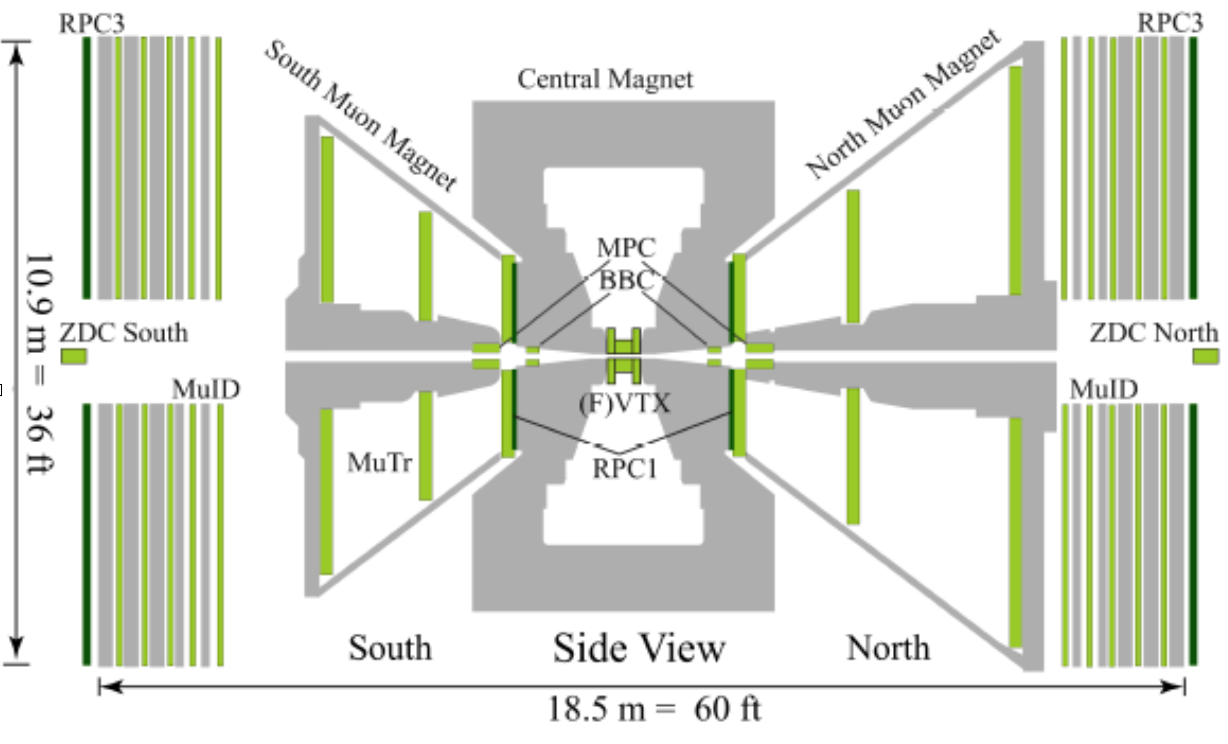
\includegraphics[width=0.55\linewidth]{figs/phenix_schematic.png}
\caption{A cross section diagram of the PHENIX detector from the incoming beam's perspective (top) and a cross section diagram of the PHENIX detector from the side (bottom). The central arm detectors are not shown in the bottom diagram~\cite{Aidala201444}.}
\label{fig:phenix_schematic}
\end{figure}

For this thesis, the relevant detectors in 2015 are the DC, PC, RICH, BBC, and FVTX. The DC, PC, and RICH are located in the mid-rapidity region relative to the collisions and are a part of  what are referred to as the Central Arms (CA) and the BBC and FVTX that are located in the forward (and backward) rapidity region relative to the collisions are a part of what is referred to as the (Forward Arms)~\cite{Adcox2003469}. 

PHENIX makes use of the three powerful magnets in order to bend charged particles' trajectories: the Central Magnet (CM), the North Muon Magnet (MMN), and the South Muon Magnet (MMS).

PHENIX has a state-of-the art Data Acquisition System (DAQ) which is capable of writing 750 MB/s of information to disk. More details about the PHENIX DAQ are found in Section \ref{sec:PHENIX_DAQ}.

For reference, Figure \ref{fig:ch3_coord_sys} depicts the PHENIX coordinate system relative to the RHIC ring. References to the cardinal directions or $x$, $y$, or $z$ are defined in relation to this figure.
\begin{figure}[!ht]
\centering
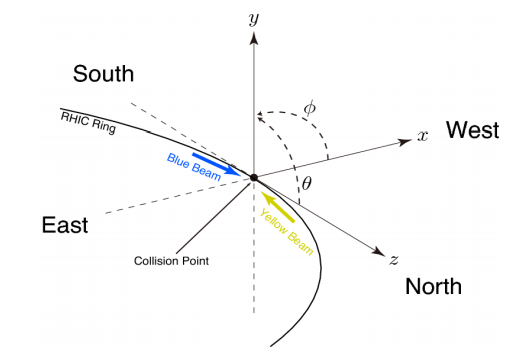
\includegraphics[width=0.55\linewidth]{figs/phenix_coord.png}
\caption{The PHENIX coordinate system. The origin is in the middle of the PHENIX detector at the collision point. North and south are parallel to beam axis. East and west are transverse to the beam axis. Central detectors have a west and an east arm on either side of the beam. Forward detectors have a north and a south arm relative to the origin.}
\label{fig:ch3_coord_sys}
\end{figure}

\subsection{PHENIX Magnet System}
 The CM has two circular coils which can be configured in the same direction (++ or $-$ $-$), the opposite direction (+$-$ or $-$ $+$), or the with the inner magnet off (+0 or $-$0). The magnets can also be run in the ``zero-field" configuration which is used for alignment purposes. Figure \ref{fig:magnet_figures} shows the magnetic field lines and strength produced by the PHENIX magnets. The magnetic field lines at mid-rapidity, $|Z| < 0.3$m on the plot, have a peak strength of $\sim$0.9 T near the beam pipe and extend out to R $\approx$ 2 m, just before the DC. The right panel of Figure \ref{fig:magnet_figures} depicts the magnetic field strength as a function of distance from the center of PHENIX. For any of the possible CM magnet configurations, the magnetic field strength is very small for $r > $ 2 m.
\begin{figure}[!ht]
\centering
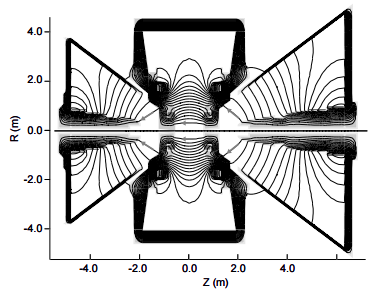
\includegraphics[width=0.45\linewidth]{figs/magnet_map.png}
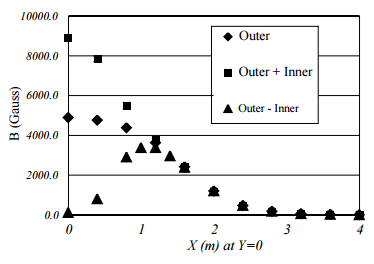
\includegraphics[width=0.45\linewidth]{figs/magnetic_field_strength.png}
\caption{PHENIX magnetic field lines from the MMS, CM, and MMN, (left) and the total magnetic field strength from the CM vs the radial distance from the center of PHENIX at $\phi$ = 0(right)~\cite{Aronson2003480}.}
\label{fig:magnet_figures}
\end{figure}
%\subsection{Forward Rapidity Detectors}
%The general design philosophy for PHENIX forward rapidity detectors 
\subsection{Beam Beam Counter}
\label{sec:bbc_det_sec}
The BBC is a forward detector used to determine the event start time, vertex, centrality, and event plane. The BBC is composed of two mirror image arrays, a South and a North Arm, that surround the beam pipe 144 cm on opposite sides of the nominal collision point just behind the Central Magnet, covering $3.0 < |\eta| < 3.9$ and 2$\pi$ radians in azimuth. Each BBC arm is made of 64 elements composed of a 3-cm length quartz Cherenkov radiator connected to a 2.5 cm diameter Hamamatsu R6178 mesh dynode PMT (photomultiplier tube), as shown in Figure \ref{fig:bbc_dector}. The outer and inner diameters of the BBC, with respect to the beam axis, are 30 cm and 10 cm, respectively.% allowing for a 1 cm clearance of the beam pipe.
\begin{figure}[!ht]
\centering
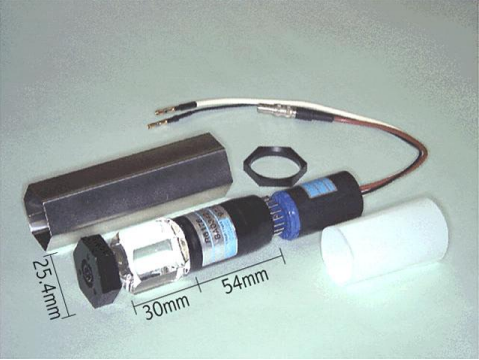
\includegraphics[width=0.45\linewidth]{figs/bbc_pmt.png}
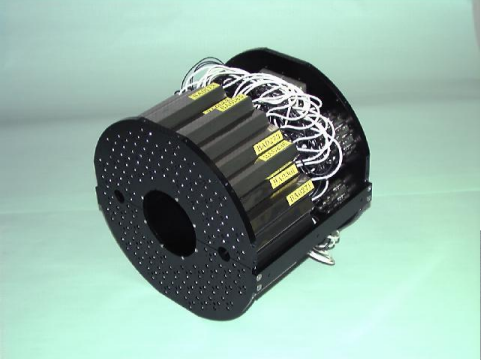
\includegraphics[width=0.45\linewidth]{figs/bbc_arm.png}
\caption{Photographs of the BBC detector. The left is of a single detector element consisting of a quartz radiator and a PMT. The right is of one of the BBC arms, consisting of 64 detector elements~\cite{Adcox2003469}.}
\label{fig:bbc_dector}
\end{figure}

%maybe add something about the BBC timing information being used to get rid of pile-up events
The BBC is used to mark the event start time for the entire PHENIX detector by averaging the emitted particles arrival time at each BBC arm. The timing difference between each arm provides an estimate of the collision's z-vertex by
\begin{equation}
z = c \frac{T_S - T_N}{2},
\end{equation}
where $T_S, T_N$ are the particle's average arrival times for each arm and $c$ is the speed of light.%check numbers here:

For \pau collisions at \sqsn = 200 GeV, the BBC has a timing resolution of $\sigma_t$ $\sim$50 ps and a corresponding $z$-vertex resolution of $\sim$1.0--2.0 cm, depending on the event charged particle multiplicity. A coarser estimate of the vertex is used during triggering, to select events of interest. Specific details about triggers are in Section \ref{sec:PHENIX_DAQ}.

The BBC also provides the centrality classification, as described in Chapter 2, Section \ref{sec:initial_condition}, of a collision event in PHENIX. Details of how BBC data is used to compute the centrality are given later in this Chapter in Section \ref{sec:central_determin}.

%\begin{figure}[!h]
%\begin{center}
%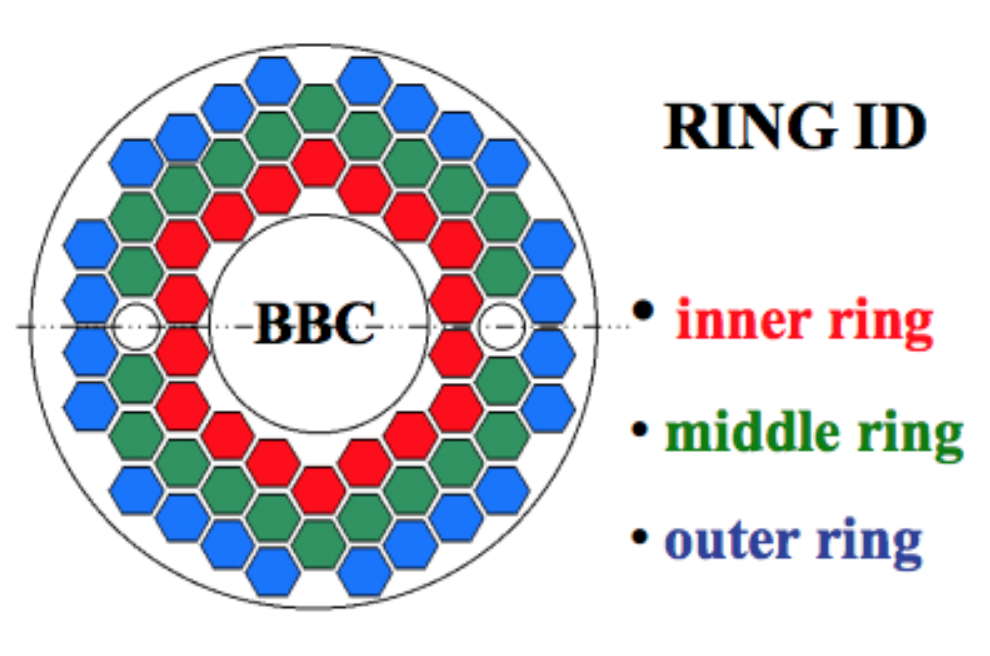
\includegraphics[width=0.4\linewidth]{figs/bbc_ring_schematic.png}
%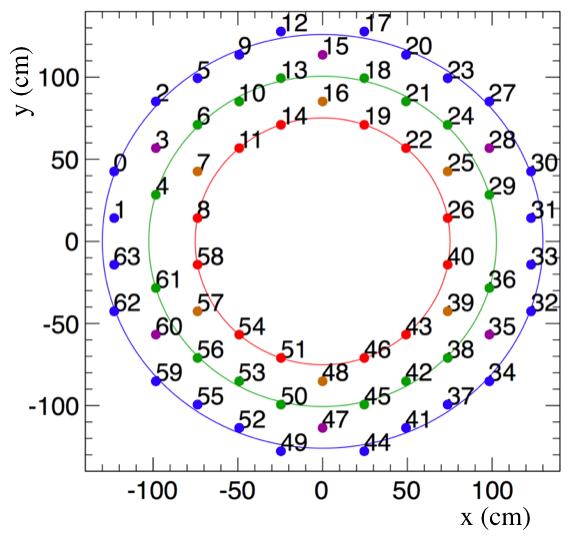
\includegraphics[width=0.4\linewidth]{figs/bbc_rings.png}
%\caption{TBA}
%\end{center}
%\end{figure}
%[LIST PHENIX forward rapidity detectors (muon ID, muon tracker, muon trigger, FVTX, RPC (maybe forget about the big list! yes it is a waste of time)]
\subsection{Forward Vertex Detector}
%[talk about how it is a new upgrade in 2012, talk about ]
The FVTX is a PHENIX detector upgrade that became operational in 2012 for taking physics data. The FVTX provides charged particle tracking, collision vertex determination, and event plane determination \cite{Aidala201444}. The FVTX consists of two identical endcaps covering a combined pseudorapidity range of 1 $<|\eta|<$ 3 and full azimuth coverage. Each endcap has four stations of silicon mini-strip sensors with a pitch of 75 $\mu$m arranged in the radial direction around the beam pipe. The basic unit of construction is a wedge that has silicon strip sensors and associated read-out chips. The inner most layer (on each side) of the FVTX has a smaller radius. Figure \ref{fig:fvtx_cutaway} is a photograph of the FVTX disks and an engineering drawing of the FVTX and its support structure. The FVTX is used in this thesis to calculate the event plane.
\begin{figure}[h!]
\centering
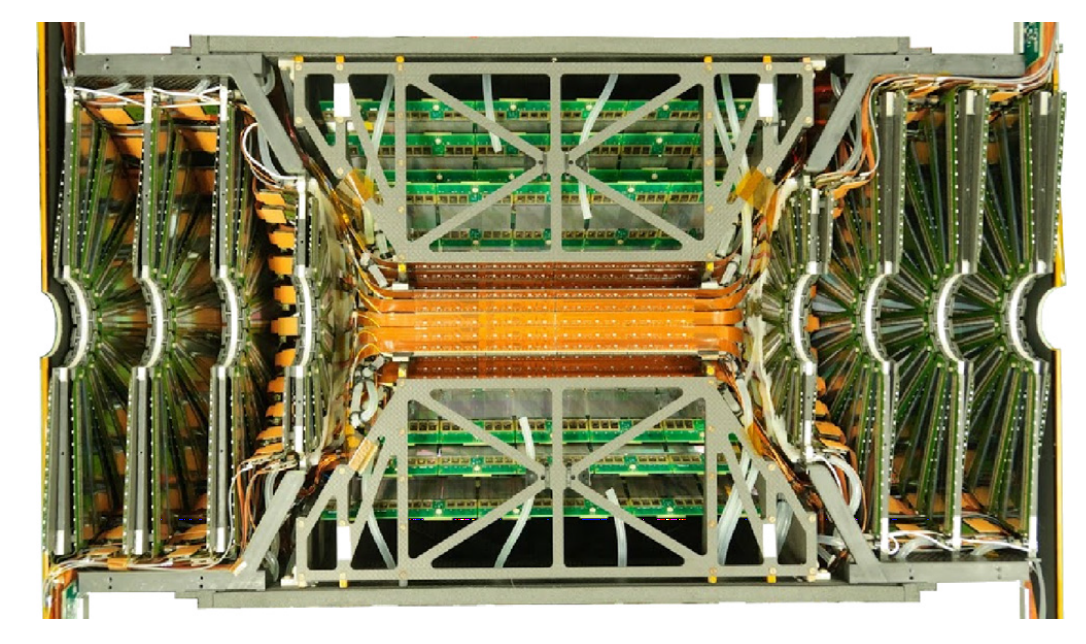
\includegraphics[width=0.45\linewidth]{figs/fvtx_cutaway.png}
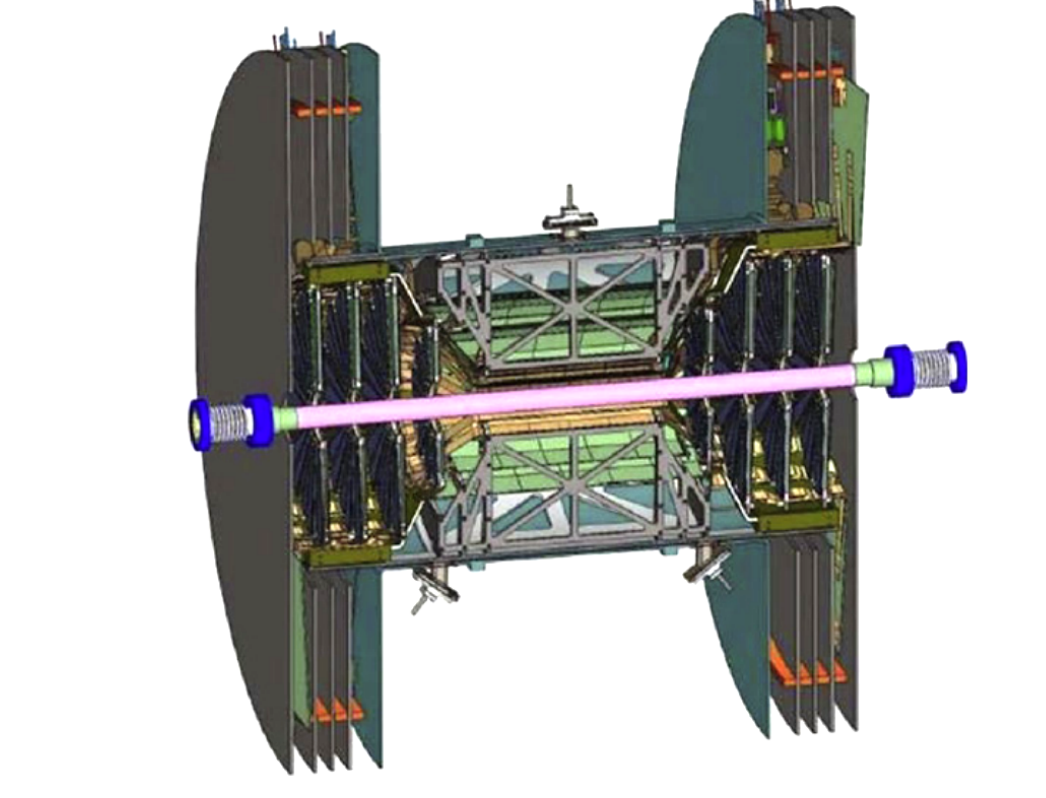
\includegraphics[width=0.45\linewidth]{figs/fvtx_diagram.png}
\caption{A photograph of half of the FVTX. In the cutaway, one sees the half disks on either end of the picture (left) and a schematic of the FVTX at a slightly different angle (right). The FVTX is only 20 cm in the $z$ direction from the PHENIX coordinate system origin (the center of each picture)~\cite{Aidala201444}.}
\label{fig:fvtx_cutaway}
\end{figure}
%\subsubsection{FVTX Clustering}
%\subsection{Midrapidity Detectors}
\subsection{Drift Chamber}
The DC consists of two gas multi-wire proportional chambers, one located in each arm. The DC is used to measure particle trajectories in the $r$-$\phi$ plane.
The DC is located $\sim$2 m from the $z$-axis, placing it in a very small residual magnetic field from the CM. Apart from the VTX, the DC is the first detector encountered by a particle produced at mid-rapidity. 

As a charged particle passes through the DC volume, a gas mixture of 50\% Argon and 50\% Ethane are ionized to create free electrons. These electrons cause a chain reaction of ionizations which are measured by an anode wire. The DC is designed in such a way that the drift velocities of the elections are predicable enough to relate time and position together. 

\begin{figure}[!ht]
\centering
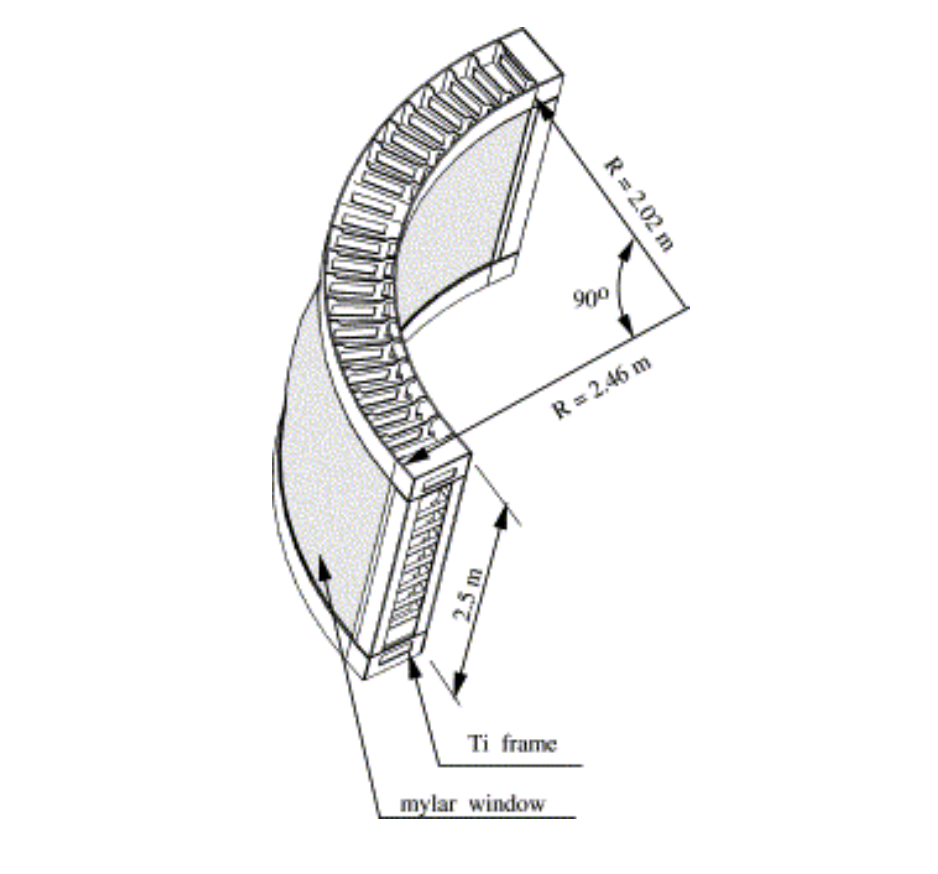
\includegraphics[width=0.45\linewidth]{figs/dc_diagram.png}
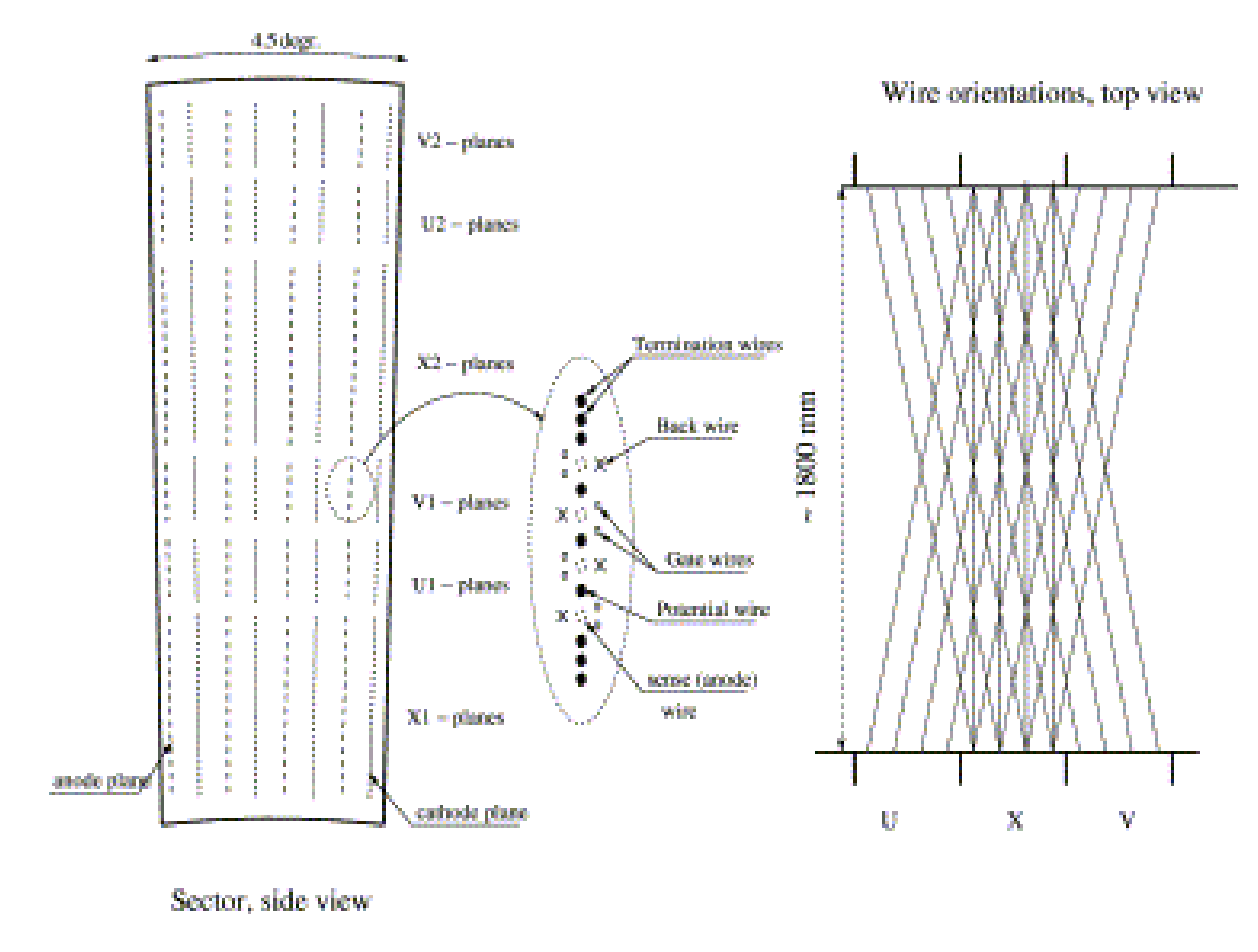
\includegraphics[width=0.45\linewidth]{figs/dc_wire_diagram.png}
\caption{A diagram of the DC titanium frame which encloses the detector (left) and a diagram of the X, U, and V wires in the DC (right)~\cite{Adcox2003469}.}
\label{fig:dc_diagram}
\end{figure}

Each identical DC arm is cylindrical in design and covers 2.5 m along the beam direction and is 0.4 m deep (in radius) as seen in the left panel in Figure \ref{fig:dc_diagram}. Each arm is divided into 20 equal sectors covering 4.5 degrees in $\phi$. Each sector contains six types of wire modules stacked radially and labeled X1, U1, V1, X2, U2, V2, respectively, from the inside out. The X wires run parallel to the beam to perform precise $\phi$ measurements while the U and V wires are set at small angles of about six degrees relative to the X wires to provide information about the $z$ position of the track. A diagram of the wire layout in each sector is shown in the right panel in Figure \ref{fig:dc_diagram}. In total, the DC consists of about 6,500 anode wires with 13,000 readout channels. The  resolution for a single wire is 165 $\mu$m in $r$-$\phi$, a single wire efficiency better than 99\%, and a spatial resolution of  2 mm in the $z$ direction.

%\clearpage
\subsection{Pad Chambers}
The PCs are multi-wire proportional chambers consisting of three separate layers of detectors measuring precise hit positions in the PHENIX tracking system. The innermost layer, PC1, is located in both the east and west arms immediately outside the DC, providing a measurement of the $x, y, z$ position at the back plane of the DC. The second layer, PC2, is located behind the RICH in the West arm only. The outer layer, PC3, is in both arms and provides a second space point on the straight line trajectories of the tracks through the detector, outside of the CM magnetic field as shown in Figure \ref{fig:magnet_figures}. PC1 hits are used as an input to the pattern recognition to reduce the track background.

\subsection{Ring Imaging Cherenkov Detector}
The RICH detector is located immediately behind the PC1 and provides the primary electron identification for PHENIX. The RICH consists of two identical detectors in the CA. Each detector contains 48 mirror panels which focus Cherenkov light onto PMTs. The RICH is filled with radiator gas, is CO$_2$, for the \pau running. The RICH provides e/$\pi$ (electron to pion) discrimination below the $\pi$ Cherenkov threshold of $\sim$4 GeV/c. Figure \ref{fig:rich_discrim_ep} shows the energy over momentum $E$/$p$ distribution in \auau \sqsn = 200 GeV collisions. The $E$ comes from the EMCAL and the $p$ comes from the DC tracks. When RICH hits are required in conjunction with DC tracks, a electron signal peak can be seen at $E$/$p$ = 1.0, as expected for electrons deposited their full energy in the EMCAL.

\begin{figure}[!ht]
\centering
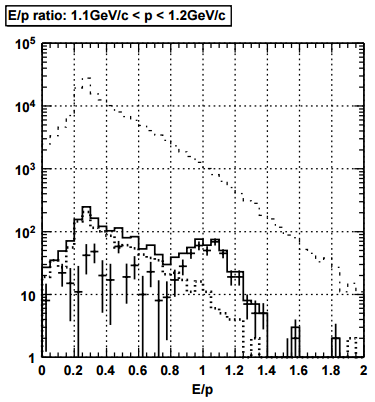
\includegraphics[width=0.55\linewidth]{figs/e_over_p_rich_discrimination.png}
\caption{Ratio of energy to momentum for all Drift Chamber tracks (dashed-dotted line), and tracks associated with RICH hits (solid line) in \auau \sqsn = 200 GeV collisions. The $p$ range is 1.1 -- 1.2 GeV/c ~\cite{Aizawa2003508}.}
\label{fig:rich_discrim_ep}
\end{figure}

\subsection{Electromagnetic Calorimeter}
The EMCAL is the outermost subsystem in the central arms and is designed primarily to measure the energies and positions of photons and electrons. It also plays a key role in particle identification, as well as providing triggering on rare events of interest. Two different EMCAL designs were utilized with 6 sectors based on a lead-scintillator design and 2 sectors based on a lead-glass design. The two different designs were chosen deliberately as each provides advantages and disadvantages; for instance the lead glass has a better energy resolution, while the lead scintillator has better linearity and timing.

\subsection{PHENIX Data Acquisition System}
\label{sec:PHENIX_DAQ}
PHENIX makes use of a fast DAQ to manage the transfer and collation of hundreds of kB of event data (per event) from over two dozen independent detector subsystems at a rate of over 6 kHz. This amounts to writing to disk hundreds of MB/s, a data writing rate which the PHENIX DAQ consistently achieves for months of constant use. 

The collection of a  Granule Timing Module (GTM), Front End Modules (FEM), and a Data Collection Modules (DCM) is known as a ``granule" and is the minimal combination of DAQ hardware sufficient for data collection, as shown in Figure \ref{fig:granule_diag}. The output data of each detector subsystem is managed by a granule. Pipelined Field Programmable Gate Arrays (FPGA) with carefully controlled dead time are used to calculate the trigger decisions. The FPGAs are fed information from the experiment. Once the FPGAs compute the trigger decision, the trigger signals are monitored by the GTM. If the trigger decision is positive, the GTMs instruct the FEMs to release their data from their buffers and send them to the DCM of their granules. If the decision is negative, the FEMs are instructed to dump the data.  Once the FEM is instructed to send its data downstream, it goes to the DCM and then is sent to the Event Builder (EvB).

\subsubsection{Triggering}
PHENIX runs 32 distinct triggers simultaneously. Each of the triggers has a scale down number to control the relative bandwidth each trigger receives. To understand the PHENIX triggers, it is useful to learn about the beam clock.

The PHENIX trigger is tied to the clock of the blue beam, one of the two counter circulating rings of which RHIC is comprised. The clock rate is fixed at 9.38 MHz and is tied to the rate at which RHIC overlaps bunches of ions in the interaction regions. Every time a bunch of ions from the blue ring overlap with a bunch of ions from the yellow ring, there is a blue clock trigger. This clock is stable by necessity of the precision required to run a complex accelerator like RHIC.

One critical trigger that is used in this analysis is the minimum bias trigger. As the name suggests, the trigger seeks to mark the detection of an ion collision while reducing to a minimum the bias to the type of the collision. To achieve this, data from the BBC are used. Although what constitutes a minimum observation varies with collision species, the BBC minimum bias trigger is generally defined as $>$0 PMTs in each arm above threshold. Not only is this condition a good indication that a ion collision occurred, it is also the minimum information necessary to calculate the collision vertex position using the BBC. The vertex information is important because it is used to select collisions which occur in the narrow range of acceptance of the current PHENIX detector configuration. This range is -10 cm $< z<$ 10 cm. For completeness, PHENIX takes BBC minimum bias triggers with z vertex cuts of 30 cm, 10 cm, and with no vertex cut. The collection of all these triggers is what is considered to be the PHENIX minimum bias trigger.

In Run 15, a high multiplicity trigger was implemented to enhance event statistics for events producing the largest number of particles (i.e. the most central, violent collisions). This trigger was given a large fraction of the bandwidth and consisted of requiring at least 35 out of 64 PMTs in the south arm (Au-going direction) of the BBC. More details about this trigger are located in Section \ref{sec:Run_15}.
\begin{table}[h!]
\centering
\caption{An example 2015 \pau at \sqsn = 200 GeV trigger configuration and parameters. A trigger's scale down number reduces its rate by 1/(1+scale down). }%numbers from run435737
    $\begin{array}{|c|c|c|c|c|}
    \hline 
    %\toprule
    %Collision Species & \pp & \pau & units & a \\ \hline
    \rm Trigger\thinspace \rm Name & \rm Scale\thinspace \rm down & \rm Trigger\thinspace \rm rate & \rm Vertex\thinspace \rm cut & \rm Part\thinspace \rm of\thinspace \rm minimum \rm bias \\ \hline
     \rm Clock & 196077 & 45 Hz  & N/A & \rm no \\ \hline
    BBC(>0\thinspace PMTs)\thinspace \rm narrowvtx& 100 &  695\thinspace Hz &  10 cm & \rm yes\\ \hline
    BBC(>0\thinspace PMTs)  & 2083 & 88\thinspace Hz &  30 cm & yes\\ \hline
    BBC(>0\thinspace PMTs)\thinspace \rm novertex& 3959 &94\thinspace Hz  &no\thinspace cut & \rm yes\\ \hline
    BBC(>35\thinspace  PMTs) & 1 & 1640\thinspace Hz &  10 cm & \rm no \\ \hline
    \end{array}$
\label{tbl:trigger_config}
\end{table}

\begin{figure}[!ht]
\centering
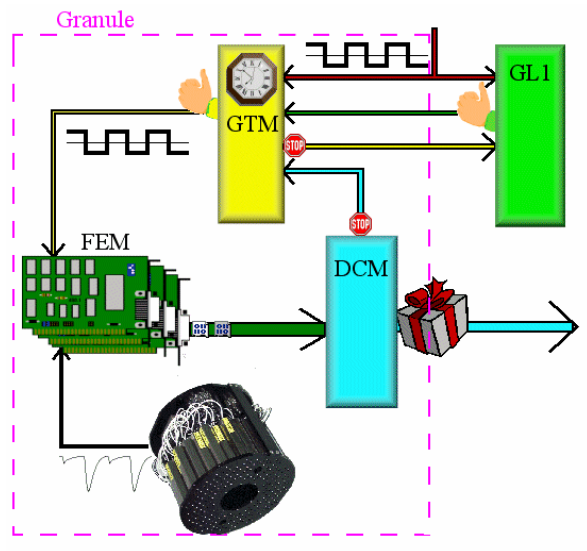
\includegraphics[width=0.55\linewidth]{figs/granule_diagram.png}
\caption{Diagram of a granule. Granules are the building blocks of the PHENIX DAQ. Each detector subsystem has at least one granule.} %Also, the GL1 has a granule.}
\label{fig:granule_diag}
\end{figure}

%\begin{figure}
%\begin{center}
%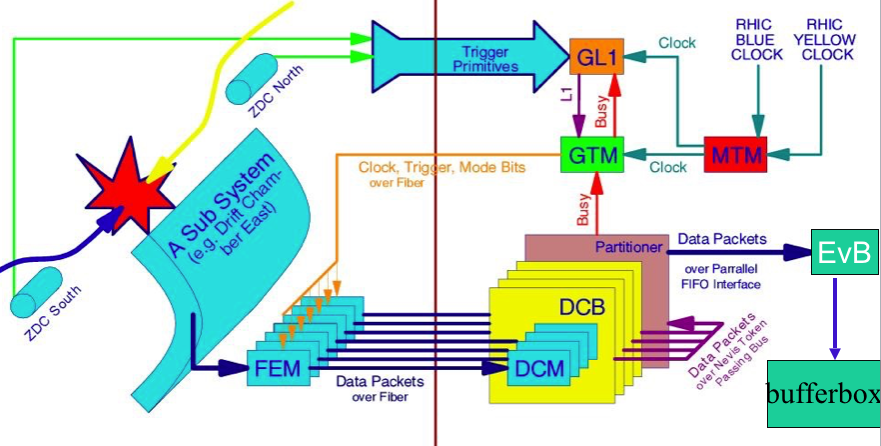
\includegraphics[width=0.75\linewidth]{figs/DAQ_diagram.png}
%\caption{Diagram of the .}
%\end{center}
%\end{figure}

\subsubsection{Event Builder}
Following the PHENIX DAQ data path, after a positive trigger decision has been sent to each of the granules, the granules' data packets are sent from that granule's FEM to the DCM and then to the event builder. It is the event builder's job to associate each granule's data packet from the same collision event into one bundle of data known as an event. The event builder consists of Sub Event Buffers (SEB), Assembly Trigger Processors (ATP), an Event Builder Controller (EBC), and a Gigabit Ethernet Switch for the communication management. The EvB transfers the data to long-term storage at the RHIC Computing Facility. Figure \ref{fig:evb_diag} shows a diagram for how these components are connected.

Granules send the data packets to the specific SEB assigned to that granule. The EBC receives global trigger information and assigns each ATP a specific collision event. The ATP then requests the data from all of the SEBs for the specific event assigned to it by the EBC. Once the ATP is successful, it writes the assembled event to disk and the EBC instructs the SEBs to flush the buffer for that event.
%This is more difficult than it may appear because event buffering means there will be multiple packets from each granule from different collision events.

\begin{figure}[h!]
\centering
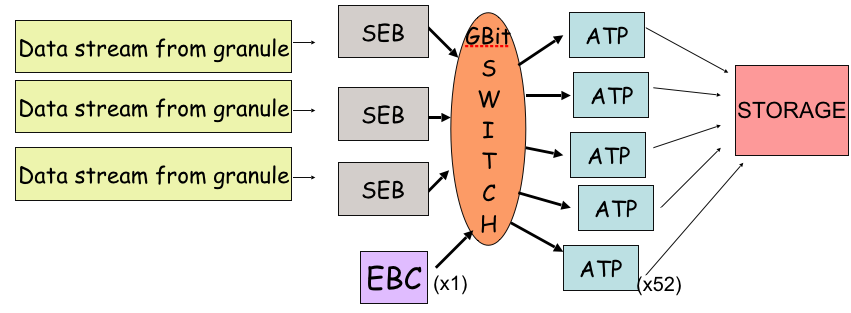
\includegraphics[width=0.73\linewidth]{figs/evb_diagram.png}
\caption{Diagram of the event builder. }\label{fig:evb_diag}
\end{figure}

%\subsubsection{Triggering}

\subsection{Run 15}
\label{sec:Run_15}
Run 15 is the RHIC running period in the year 2015, which marks the fifteenth in consecutive years of RHIC running since the year 2000. Run 15 began in January 2015 and ended in June of 2015. There were approximately eleven weeks of good physics data taken, approximately five weeks of polarized \pp collisions at \sqs = 200 GeV, approximately five weeks of polarized \pau collisions at \sqsn = 200 GeV, and approximately of research viable \pal collisions \sqsn = 200 GeV. Of interest to this thesis are the \pp and \pau datasets. 
\begin{table}[h!]
\caption{Some relevant RHIC parameters from Run 15.}
\begin{center}
    \begin{tabular}{| l | l | l | l |}
    \hline
    Collision Species & \pp & \pau & units\\ \hline
    Total Particle Energy & 100.2 & 103.9 + 100.0  & GeV/nucleon \\ \hline
    Ions per Bunch & 225 &  225 + 1.6 & number $\times10^{9}$ \\ \hline
    Number of Bunches & 111& 111 & number\\ \hline
    Luminosity Average Per Fill& $6,300\times10^{28}$ & $45 \times10^{28}$&$\rm cm^{-2}s^{-1}$ \\ \hline
    Total Delivered Luminosity & 382  & 1.27 & $\rm pb^{-1}$ \\ \hline
    Average Fill Lifetime & 8 & 7 & hours\\ \hline
    \end{tabular}
\end{center}
\end{table}

In addition to providing the minimum bias as trigger for Run 15, the BBC was used to implement a high-multiplicity trigger in order to enhance the amount of the top $5\%$ highest multiplicity events. The high-multiplicity trigger requires at least 35 of the 64 BBC south arm.  PMTs to be above threshold in a given event to be satisfied. The relevant BBC arm for \pau is the south arm since that is the Au-going direction so the multiplicity is much higher in the south arm. The central trigger enhancement can be seen in Figure \ref{fig:pau_centrality_trig}. 

%Also, the BBC was used to determine the event centrality by summing the charge collection of each
%BBC element; it is assumed the larger the charge collection the more central the
%event. This will be further discussed in Sec. (TBA) Moreover, the BBC can measure
%event plane using. For further BBC event plane calculation details see section (TBA).

\begin{figure}[!ht]
\centering
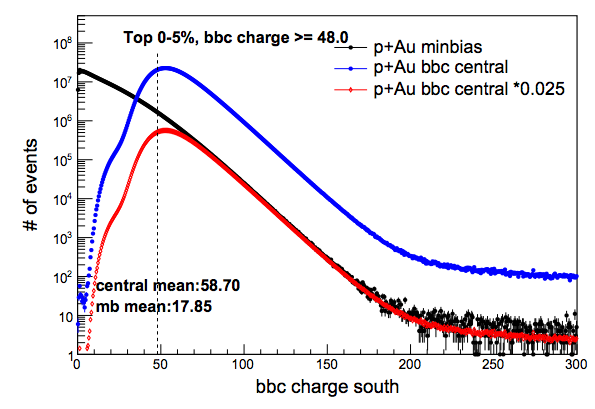
\includegraphics[scale=0.55]{figs/pAu_centrality_trigger.png}
\caption{The distribution of BBC charges in \pau at \sqsn 200 GeV events for different triggers. The black curve is the distribution of charges for the minimum bias trigger. The blue and red curves are the distributions of charges for the high multiplicity trigger. The red curve being scaled by a factor of 1/40 to show agreement with the black curve. The definition of the top 5\% more central events are BBC south charges $>=$ 48.0. The plot shows the large enhancement of the number of 0-5\% centrality events that are gained using the high multiplicity trigger compared to the number of 0-5\% centrality from the minimum bias trigger alone.}
\label{fig:pau_centrality_trig}
\end{figure}

\subsubsection{Beam Collision Geometry}
\label{sec:ch2_beam_col_geo}
For the 2015 \pau collisions at \sqsn = 200 GeV running, The RHIC's blue and yellow beams were not in perfect accordance to the PHENIX coordinate system. This was manifested in two separate ways. First of all, the collision vertex is significantly offset from the z-axis to which all of the PHENIX detectors are aligned. This is a typical situation in PHENIX datasets but it must be addressed. The other effect, and the more significant of the two, comes from the fact that the beams are colliding at an angle of 3.6 mRad in the $x$-$z$ plane, as illustrated in Figure \ref{fig:beam_angle}. 

The reason for this is because of the accelerator ring magnet requirements for running \pau at \sqsn = 200 GeV at RHIC. It is highly desirable to have the beams at equal energy per nucleon, and since the proton and the Au have different $Z$/$A$ ratios, the magnets require different settings to control the beams. The final D$X$ magnet constrains both beams and moves them to cross at the interaction region in the middle of PHENIX. The beam angle is needed to offset the beams in the D$X$ magnet field~\cite{BNL_Run15_Operations}.

\begin{figure}[!ht]
\centering
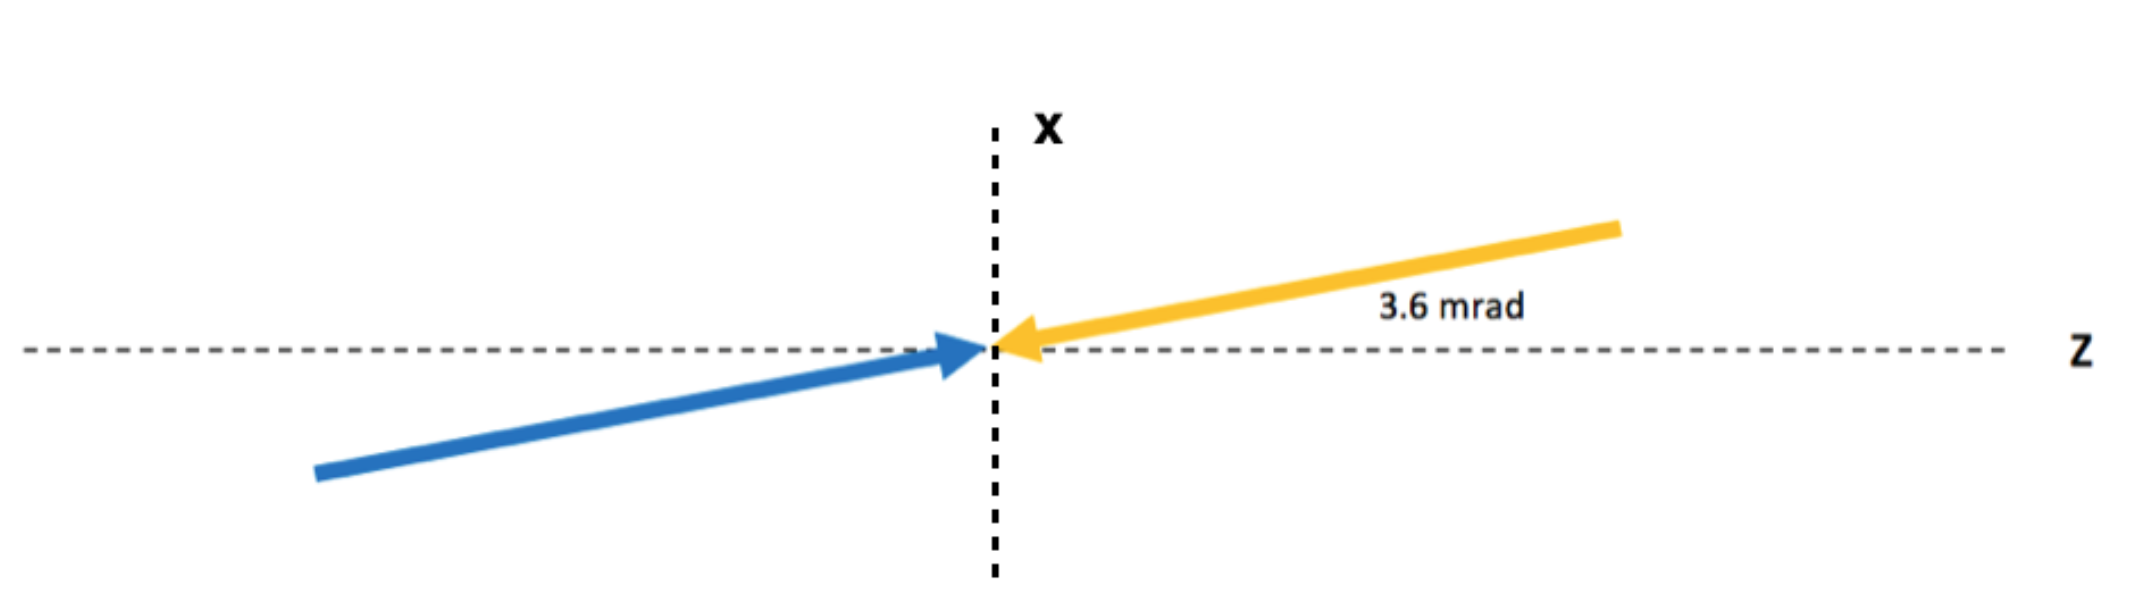
\includegraphics[width=0.85\linewidth]{figs/beam_angle.png}
\caption{A vector diagram illustrating the yellow and blue beam angle confirmation relative to the PHENIX coordinate system.}
\label{fig:beam_angle}
\end{figure}

The collision vertex in $x$ and $y$ is known as the beam center. The beam center varies over the course of data taking but its values on average are $(x,y) = (0.206,0.065) (\rm cm)$. The distribution of z-vertices from collision events can be see in Figure \ref{fig:bbc_z_vtx_dist}. Due to the fact that the beams are colliding at an angle in the $x$-$z$ plane, the $x$-component of the beam center will have a z-vertex dependence with a slope of -0.0036 cm of $x$ per 1 cm of $z$.
Apart from how the beam angle effects the beam center values, it also violates the expectation of a uniform $\phi$ distribution of particles with respect to PHENIX detectors. PHENIX detectors are designed and aligned, with respect to the PHENIX coordinate system, with the expectation of geometric symmetry. A significant beam collision angle with respect to PHENIX detectors would be equivalent to PHENIX detectors being tilted, which would violate geometric symmetry.
The physics analysis described in this thesis is sensitive to these beam geometry effects. A discussion on how to account for these effects will be in Chapter 4.

% The reason a non-ideal beam geometry 
%creates an east west v2 measurement difference is because of the assumption that event plane angle is azimuthally
% isotropic during the event plane flattening calibration. In the translated and rotated frame where the beams aligned with the z-axis the event plane distribution would be %uniform, but in the lab frame the event plane distribution in $\phi$ would have regions of enhancement and reduction.

\begin{figure}[h!]
\centering
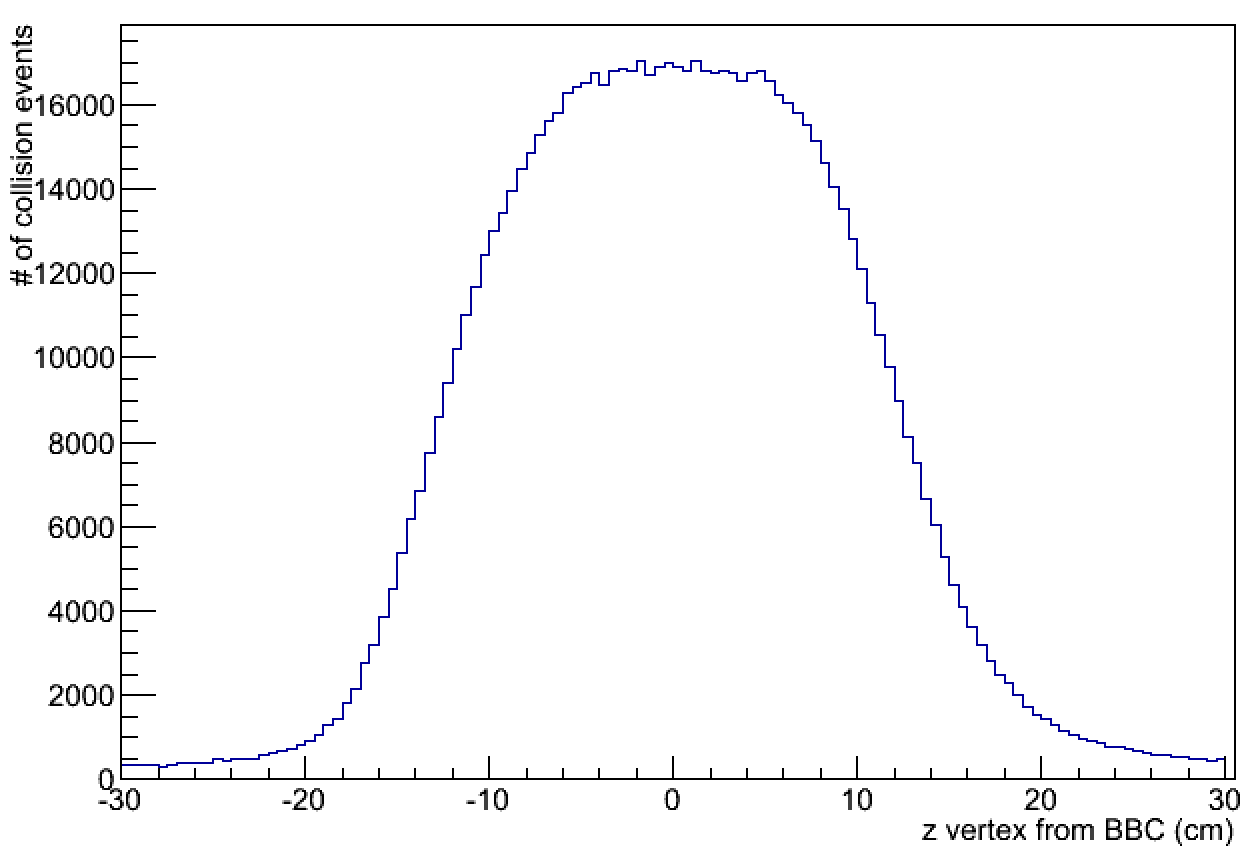
\includegraphics[width=0.65\linewidth]{figs/bbc_z_vertex_dist.png}
\caption{The BBC $z$-vertex distribution in a typical \pau run for different triggers a described in Table \ref{tbl:trigger_config}.  The teal curve is the BBC($>$0\thinspace PMTs)\thinspace novertex trigger, the blue is the BBC($>$0\thinspace PMTs), and the magneta is the BBC($>$0\thinspace PMTs)\thinspace narrowvertex.}
\label{fig:bbc_z_vtx_dist}
\end{figure}

\subsection{Centrality Determination}
\label{sec:central_determin}
The centrality determination is done by adding up all BBC South (BBCs) (Au-going direction) PMT charges for every event and then splitting up that distribution into equivalent centrality bins. This procedure, which is the same used for \dau, as documented in Ref~\cite{PhysRevC.90.034902}, is used to associate a centrality bin with number of binary collisions from Monte Carlo Glauber (MC-Glauber), as discussed in Chapter 2 Section \ref{sec:ch2_mc_glaub}. An example of such MC-Glauber event for \dau is seen in Figure \ref{fig:glauber_event_display}.  
\label{centrality_determination}
\begin{figure}[!ht]
\centering
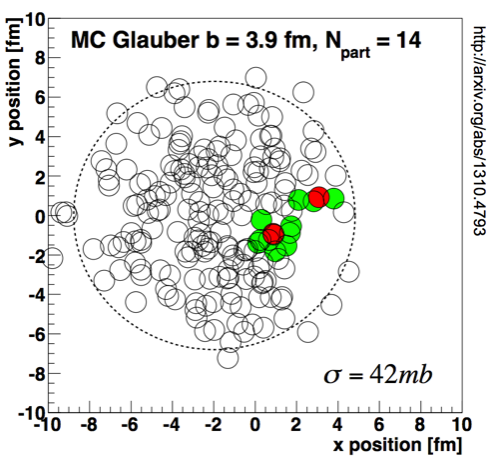
\includegraphics[width=0.5\linewidth]{figs/glauber_event_display.png}
\caption{A Monte Carlo Glauber d+Au event display. Each circle is a nucleon and filled circles are nucleons with at least one collision. The red nucleons are from the projectile (deuteron) and the green nucleons are participants from the target (gold)~\cite{PhysRevC.90.034902}.}
\label{fig:glauber_event_display}
\end{figure}

In this procedure, the total BBC charge is assumed to be proportional to the number of binary collisions in a \pau collision. Fluctuations are described probabilistically via the Negative Binomial Distribution (NBD) as defined:
\begin{equation}
   \textrm{NBD}(x;\mu,\kappa) = \left(1+\frac{\mu}{\kappa}\right)\frac{(\kappa+x-1)!}{x!(\kappa-1)!}\left(\frac{\mu}{\mu+\kappa}\right)^x
\end{equation}
where $\mu$ and $\kappa$ are the mean and positive exponent parameters. The NBD was chosen for this situation due to the linear scaling of the NBD parameters, i.e. randomly sampling from $n$ NBD($\mu$,$\kappa$) becomes NBD($n\mu$,$n\kappa$). We fold the MC-Glauber with the NBD such that the charge distribution is described as
\begin{equation}
   P(x) = \sum^{N_{COL}\textrm{max}}_{n=1} \textrm{Gl}(n)\times \textrm{NBD}(x;n\mu;n\kappa),
\end{equation}
where $x$ is the BBCs charge and Gl($n$) is the event normalized Glauber distribution~\cite{PhysRevC.90.034902}. The two parameters $\mu$ and $\kappa$ are fit to the experimental BBCs charge distribution, as shown in Figure \ref{fig:cent_determination_plot}. This figure shows good agreement between the data and the MC-Glauber + NBD fit. The best fit NBD parameters are $\mu$ = 3.14, $\kappa$ = 0.47. 

There is a deviation at small BBCs charge because the minimum bias trigger is inefficient due to the fact that a PMT must be hit in both the BBC South and North. The bottom panel of Figure \ref{fig:cent_determination_plot} is the ratio of the data to the theory curve shows that the agreement is good at a charge of 10 and greater. This ratio is fit to determine the minimum bias trigger efficiency as it ``turns on." This fit has good agreement with the turn-on curve which can be integrated to determine that the minimum bias trigger is 84\% $\pm$ 4\% efficient. By combining the measured \pau cross section with the 84\% trigger efficiency, we determine the the total inelastic \pau cross section $\sigma$ = 1.76 b. Thus, centrality is defined as a percentage of the total inelastic cross section.

\begin{figure}[!h]
\centering
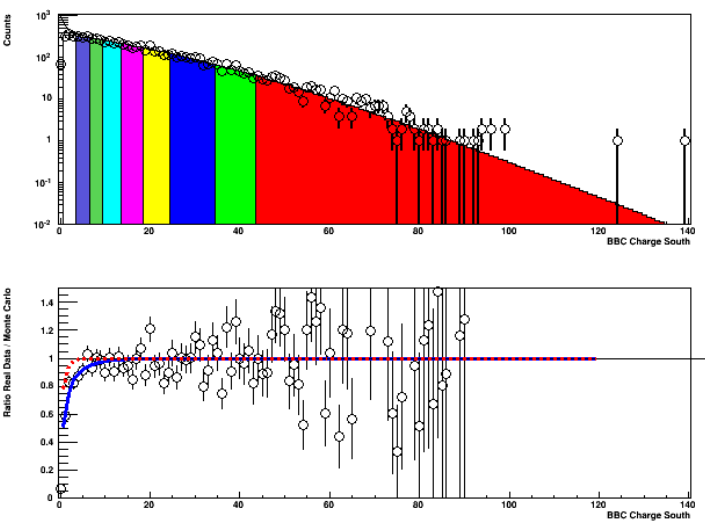
\includegraphics[width=0.65\linewidth]{figs/centrality_determination.png}
\caption{Real data for BBCs charge shown as open circles and MC-Glauber + NBD (top). The colors correspond to the various percentiles relative to the total inelastic \pau cross section, from right to left: 0--5$\%$, 5--10\%, 10--20\%, 20--30\%, 30--40\%, 40--50\%, 50--60\%, 60-70\%, and 70-84\%. The blue and red curves correspond to the minimum bias trigger efficiency in all inelastic collisions and inelastic collisions producing a particle at mid-rapidity, respectively (bottom).}
\label{fig:cent_determination_plot}
\end{figure}

%It is important to note that an extra correction is applied to the centrality determination in the form of centrality bias factors. This centrality bias is 

\iffalse

\begin{figure}[!h]
\begin{center}
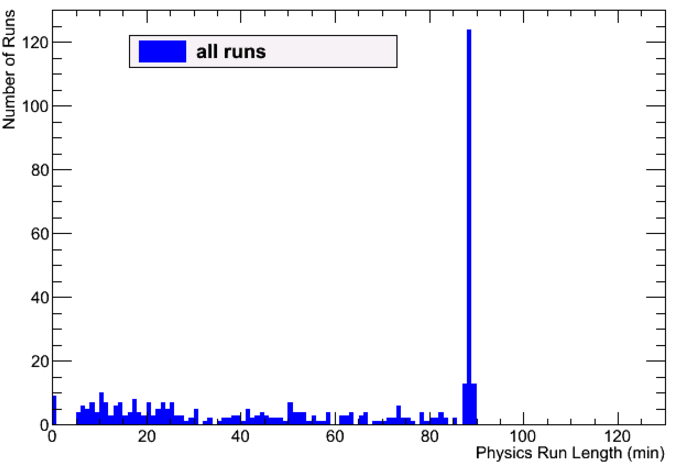
\includegraphics[width=0.65\linewidth]{figs/hruntime.png}
\caption{The distribution of the length of physics runs.}
\end{center}
\end{figure}

\begin{figure}[!h]
\begin{center}
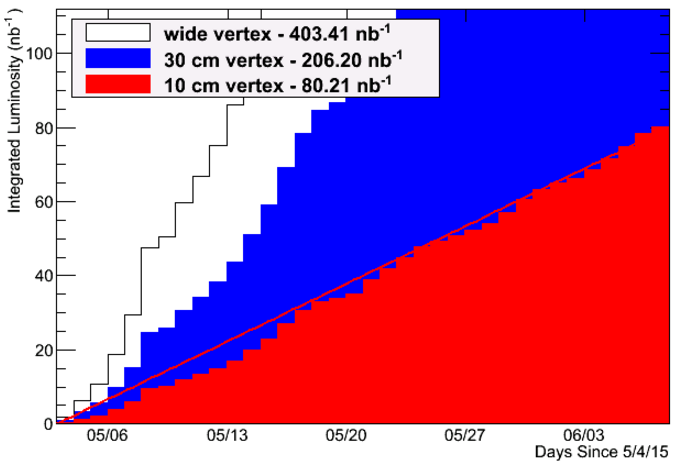
\includegraphics[width=0.65\linewidth]{figs/integrated_luminosity.png}
\caption{Integrated luminosity from the \pau dataset.}
\end{center}
\end{figure}

\fi

%\section{Event Reconstruction and Characterization}
%[not sure about this section]
%\subsection{Central Arm Tracking}
%\begin{figure}
%\begin{center}
%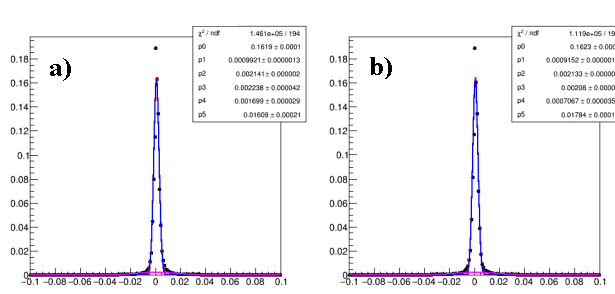
\includegraphics[scale=0.35]{figs/pc3dphi.png}
%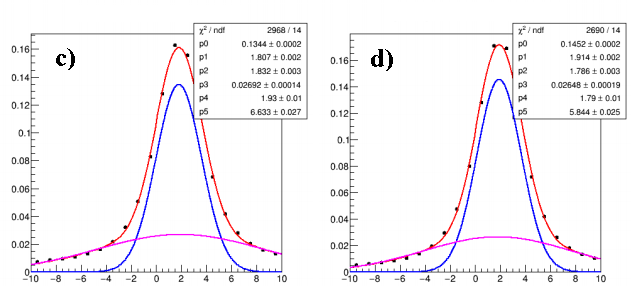
\includegraphics[scale=0.35]{figs/pc3dz.png}
%\end{center}
%\caption{TBA}
%\end{figure}
%\subsection{CNT Tracks Simulation}
%\subsection{Centrality Determination}
%\subsection{Vertex Determination}
%\begin{figure}
%\begin{center}
%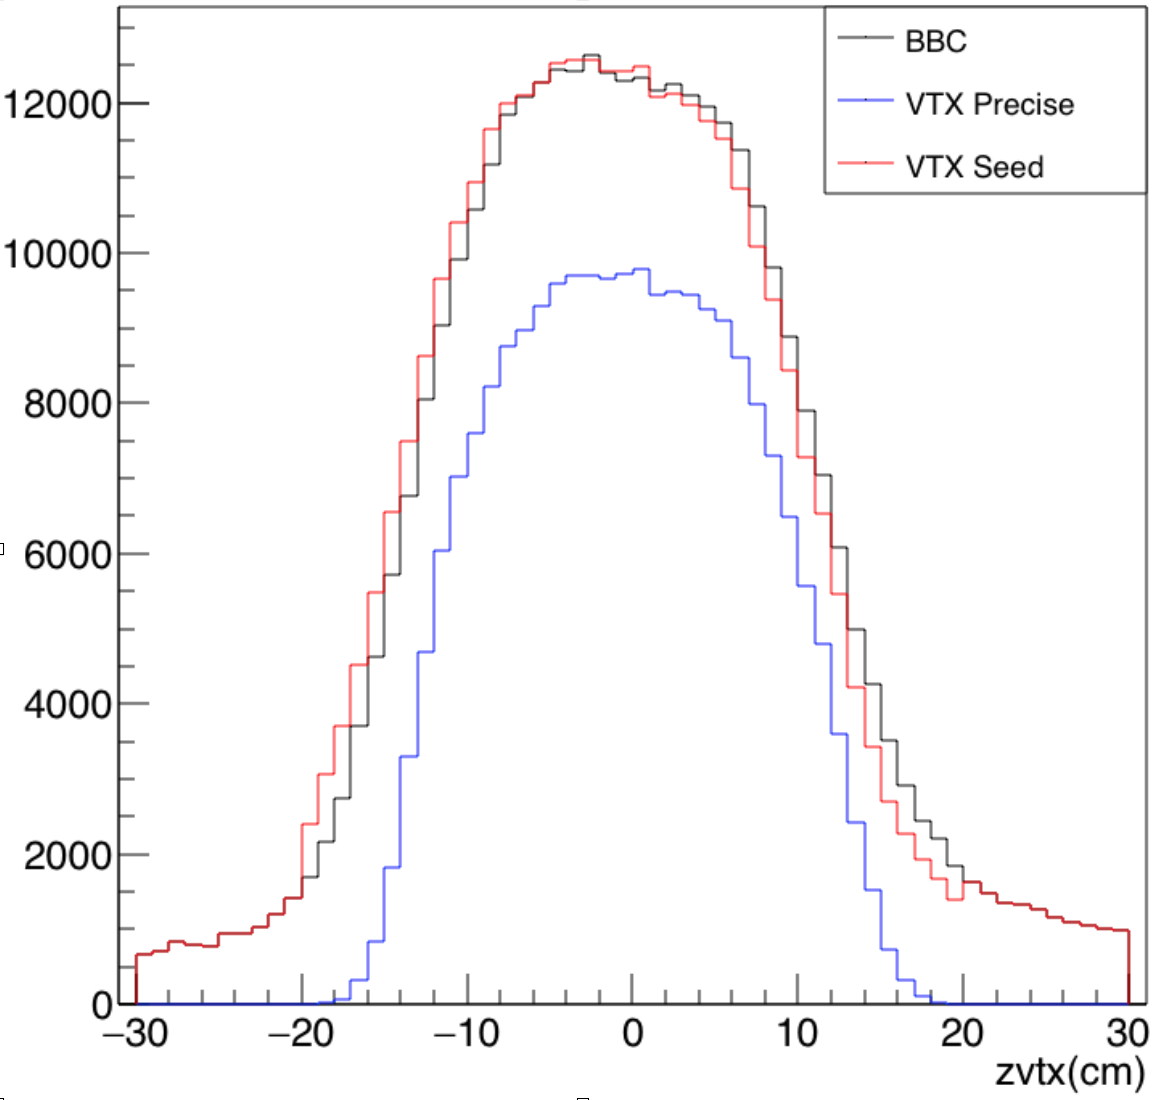
\includegraphics[scale=0.35]{figs/zvtx_distributions.png}
%\end{center}
%\caption{TBA}
%\end{figure}
%type type type type yo da lay dee hoo yo da lay yo da lay hoooooooo....
% and in her eyes, you see nothing. no sign of love behind the tears, cried for no one. a love that should have lasted years...

%\section{Run15 pAu Dataset}
%\subsection{Beam Geometry Effects}
%\begin{figure}
%\begin{center}
%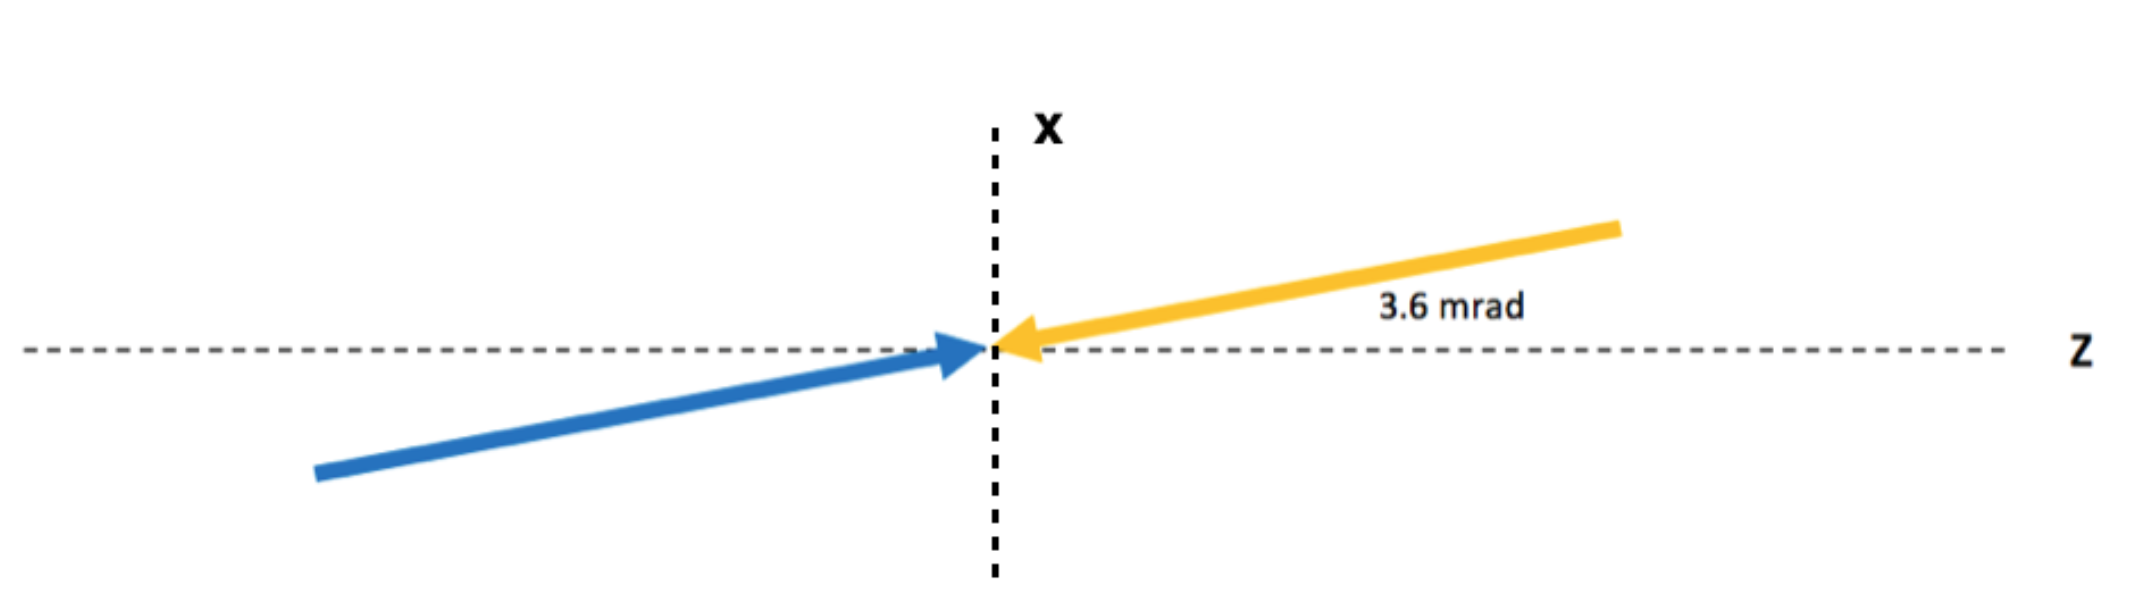
\includegraphics[width=0.65\linewidth]{figs/beam_angle.png}
%\caption{A vector diagram illustrating the yellow and blue beam angle.}
%\end{center}
%\end{figure}


